\documentclass{article}
\usepackage[margin=1in]{geometry}
\usepackage[linesnumbered,ruled,vlined]{algorithm2e}
\usepackage{amsfonts}
\usepackage{amsmath}
\usepackage{amssymb}
\usepackage{amsthm}
\usepackage{enumitem}
\usepackage{fancyhdr}
\usepackage{hyperref}
\usepackage{minted}
\usepackage{multicol}
\usepackage{pdfpages}
\usepackage{standalone}
\usepackage[many]{tcolorbox}
\usepackage{tikz-cd}
\usepackage{transparent}
\usepackage{xcolor}
% \tcbuselibrary{minted}

\author{Nathan Solomon}

\newcommand{\fig}[1]{
    \begin{center}
        \includegraphics[width=\textwidth]{#1}
    \end{center}
}

% Math commands
\renewcommand{\d}{\mathrm{d}}
\DeclareMathOperator{\id}{id}
\DeclareMathOperator{\im}{im}
\DeclareMathOperator{\proj}{proj}
\DeclareMathOperator{\Span}{span}
\DeclareMathOperator{\Tr}{Tr}
\DeclareMathOperator{\tr}{tr}
\DeclareMathOperator{\ad}{ad}
\DeclareMathOperator{\ord}{ord}
%%%%%%%%%%%%%%% \DeclareMathOperator{\sgn}{sgn}
\DeclareMathOperator{\Aut}{Aut}
\DeclareMathOperator{\Inn}{Inn}
\DeclareMathOperator{\Out}{Out}
\DeclareMathOperator{\stab}{stab}

\newcommand{\N}{\ensuremath{\mathbb{N}}}
\newcommand{\Z}{\ensuremath{\mathbb{Z}}}
\newcommand{\Q}{\ensuremath{\mathbb{Q}}}
\newcommand{\R}{\ensuremath{\mathbb{R}}}
\newcommand{\C}{\ensuremath{\mathbb{C}}}
\renewcommand{\H}{\ensuremath{\mathbb{H}}}
\newcommand{\F}{\ensuremath{\mathbb{F}}}

\newcommand{\E}{\ensuremath{\mathbb{E}}}
\renewcommand{\P}{\ensuremath{\mathbb{P}}}

\newcommand{\es}{\ensuremath{\varnothing}}
\newcommand{\inv}{\ensuremath{^{-1}}}
\newcommand{\eps}{\ensuremath{\varepsilon}}
\newcommand{\del}{\ensuremath{\partial}}
\renewcommand{\a}{\ensuremath{\alpha}}

\newcommand{\abs}[1]{\ensuremath{\left\lvert #1 \right\rvert}}
\newcommand{\norm}[1]{\ensuremath{\left\lVert #1\right\rVert}}
\newcommand{\mean}[1]{\ensuremath{\left\langle #1 \right\rangle}}
\newcommand{\floor}[1]{\ensuremath{\left\lfloor #1 \right\rfloor}}
\newcommand{\ceil}[1]{\ensuremath{\left\lceil #1 \right\rceil}}
\newcommand{\bra}[1]{\ensuremath{\left\langle #1 \right\rvert}}
\newcommand{\ket}[1]{\ensuremath{\left\lvert #1 \right\rangle}}
\newcommand{\braket}[2]{\ensuremath{\left.\left\langle #1\right\vert #2 \right\rangle}}

\newcommand{\catname}[1]{{\normalfont\textbf{#1}}}

\newcommand{\up}{\ensuremath{\uparrow}}
\newcommand{\down}{\ensuremath{\downarrow}}

% Custom environments
\newtheorem{thm}{Theorem}[section]

\definecolor{probBackgroundColor}{RGB}{250,240,240}
\definecolor{probAccentColor}{RGB}{140,40,0}
\newenvironment{prob}{
    \stepcounter{thm}
    \begin{tcolorbox}[
        boxrule=1pt,
        sharp corners,
        colback=probBackgroundColor,
        colframe=probAccentColor,
        borderline west={4pt}{0pt}{probAccentColor},
        breakable
    ]
    \color{probAccentColor}\textbf{Problem \thethm.} \color{black}
} {
    \end{tcolorbox}
}

\definecolor{exampleBackgroundColor}{RGB}{212,232,246}
\newenvironment{example}{
    \stepcounter{thm}
    \begin{tcolorbox}[
      boxrule=1pt,
      sharp corners,
      colback=exampleBackgroundColor,
      breakable
    ]
    \textbf{Example \thethm.}
} {
    \end{tcolorbox}
}

\definecolor{propBackgroundColor}{RGB}{255,245,220}
\definecolor{propAccentColor}{RGB}{150,100,0}
\newenvironment{prop}{
    \stepcounter{thm}
    \begin{tcolorbox}[
        boxrule=1pt,
        sharp corners,
        colback=propBackgroundColor,
        colframe=propAccentColor,
        breakable
    ]
    \color{propAccentColor}\textbf{Proposition \thethm. }\color{black}
} {
    \end{tcolorbox}
}

\definecolor{thmBackgroundColor}{RGB}{235,225,245}
\definecolor{thmAccentColor}{RGB}{50,0,100}
\renewenvironment{thm}{
    \stepcounter{thm}
    \begin{tcolorbox}[
        boxrule=1pt,
        sharp corners,
        colback=thmBackgroundColor,
        colframe=thmAccentColor,
        breakable
    ]
    \color{thmAccentColor}\textbf{Theorem \thethm. }\color{black}
} {
    \end{tcolorbox}
}

\definecolor{corBackgroundColor}{RGB}{240,250,250}
\definecolor{corAccentColor}{RGB}{50,100,100}
\newenvironment{cor}{
    \stepcounter{thm}
    \begin{tcolorbox}[
        enhanced,
        boxrule=0pt,
        frame hidden,
        sharp corners,
        colback=corBackgroundColor,
        borderline west={4pt}{0pt}{corAccentColor},
        breakable
    ]
    \color{corAccentColor}\textbf{Corollary \thethm. }\color{black}
} {
    \end{tcolorbox}
}

\definecolor{lemBackgroundColor}{RGB}{255,245,235}
\definecolor{lemAccentColor}{RGB}{250,125,0}
\newenvironment{lem}{
    \stepcounter{thm}
    \begin{tcolorbox}[
        enhanced,
        boxrule=0pt,
        frame hidden,
        sharp corners,
        colback=lemBackgroundColor,
        borderline west={4pt}{0pt}{lemAccentColor},
        breakable
    ]
    \color{lemAccentColor}\textbf{Lemma \thethm. }\color{black}
} {
    \end{tcolorbox}
}

\definecolor{proofBackgroundColor}{RGB}{255,255,255}
\definecolor{proofAccentColor}{RGB}{80,80,80}
\renewenvironment{proof}{
    \begin{tcolorbox}[
        enhanced,
        boxrule=1pt,
        sharp corners,
        colback=proofBackgroundColor,
        colframe=proofAccentColor,
        borderline west={4pt}{0pt}{proofAccentColor},
        breakable
    ]
    \color{proofAccentColor}\emph{\textbf{Proof. }}\color{black}
} {
    \qed \end{tcolorbox}
}

\definecolor{noteBackgroundColor}{RGB}{240,250,240}
\definecolor{noteAccentColor}{RGB}{30,130,30}
\newenvironment{note}{
    \begin{tcolorbox}[
        enhanced,
        boxrule=0pt,
        frame hidden,
        sharp corners,
        colback=noteBackgroundColor,
        borderline west={4pt}{0pt}{noteAccentColor},
        breakable
    ]
    \color{noteAccentColor}\textbf{Note. }\color{black}
} {
    \end{tcolorbox}
}


\fancyhf{}
\setlength{\headheight}{24pt}

\date{\today}
\title{Math 151A Homework \#6}

\begin{document}
\maketitle

\begin{prob}
\end{prob}
\begin{enumerate}[label=(\alph*)]
    \item For any $x \in [a,b]$, there exists $\xi \in [x_0, x]$ such that
        \[ f(x) = f(x_0) + f'(x_0)(x-x_0) + \frac{f''(x_0)}{2} (x-x_0)^2 + \frac{f'''(x_0)}{6} (x-x_0)^3 + \frac{f''''(\xi)}{24} (x-x_0)^4. \]
    \item \begin{align*}
        f(x_0+h) &= f(x_0) + f'(x_0)h + \frac{f''(x_0)h^2}{2} + \frac{f'''(x_0)h^3}{6} + \frac{f''''(\xi_1)h^4}{24} \\
        f(x_0-h) &= f(x_0) - f'(x_0)h + \frac{f''(x_0)h^2}{2} - \frac{f'''(x_0)h^3}{6} + \frac{f''''(\xi_2)h^4}{24} \\
        \frac{f(x_0-h)+f(x_0+h)-2f(x_0)}{h^2} &= f''(x_0)+ \frac{h^2}{24} \left( f''''(\xi_1) + f''''(\xi_2) \right) \\
                                              &= f''(x_0) + \frac{h^2}{24} f^{(4)}(\xi_3).
    \end{align*}
\item As $h$ goes to zero, $f''''(\xi_1)$ and $f''''(\xi_2)$ both approach a constant, so when calculating $f''(x_0)$, the error term is $O(h^2)$.
\end{enumerate}

\bigskip
\begin{prob}
\end{prob}
The total error bound is
\[ \abs{ - \frac{h^2M}{6} } + \abs{ \frac{\varepsilon}{h} } = \frac{h^2 M}{6} + \frac{\varepsilon}{h}, \]
since $h$ and $\varepsilon$ are both positive. If we treat $\varepsilon$ and $\abs{M}$ as constants, then the total error is a smooth function of $h \in (0, \infty)$, meaning we can calculate the minima and maxima by looking at the points where the derivative of the error bound with respect to $h$ is zero.
\[ \frac{\partial}{\partial h} \left( \frac{h^2 M}{6} + \frac{\varepsilon}{h} \right) = \frac{h M}{3} - \frac{\varepsilon}{h^2} = 0, \]
so $h^3 M/3 = \varepsilon$, so $h = \sqrt[3]{3 \varepsilon / M}$. This is the only real solution to the equation above, and the second derivative of the error bound with respect to $h$ is always positive, so $h = \sqrt[3]{3 \varepsilon / M}$ minimizes the error bound.
\par
Note that I have assumed $\varepsilon$ does not depend on $h$, because the expression we are given is an upper bound on the error, not an exact value of the error. Because of that, I assumed $\varepsilon_1$ and $\varepsilon_2$ are upper bounds on the roundoff errors, not exact values of the roundoff errors.

\bigskip
\begin{prob}
\end{prob}
\begin{enumerate}[label=(\alph*)]
    \item
    \[ f'(x_0) = \frac{f(x_0+h/2)-f(x_0-h/2)}{h} - \left( \frac{h^2}{24} f'''(x_0) + \frac{h^4}{1920} f^{(5)}(\xi_1) \right). \]
\item For some $\xi_3 \in [x_0-h, x_0+h]$, \begin{align*}
    4f'(x_0) &= 4 \cdot \frac{f(x_0+h/2)-f(x_0-h/2)}{h} - \left( \frac{h^2}{6} f'''(x_0) + \frac{h^4}{480} f^{(5)}(\xi_1) \right) \\
    f'(x_0) &= \frac{f(x_0+h)-f(x_0-h)}{2h} - \left( \frac{h^2}{6} f'''(x_0) + \frac{h^4}{120} f^{(5)}(\xi_2) \right) \\
    3f'(x_0) &= \frac{f(x_0+h) + 8f(x_0+h/2)-8f(x_0-h/2)-f(x_0-h)}{2h} - \frac{h^4}{480} \left( f^{(5)}(\xi_1) + 4f^{(5)}(\xi_2) \right) \\
    &= \frac{f(x_0+h) + 8f(x_0+h/2)-8f(x_0-h/2)-f(x_0-h)}{2h} - \frac{h^4}{480} \left( 5 f^{(5)}(\xi_3) \right) \\
    f'(x_0) &= \frac{f(x_0+h) + 8f(x_0+h/2)-8f(x_0-h/2)-f(x_0-h)}{6h} - \frac{h^4}{288} f^{(5)}(\xi_3). \\
\end{align*}
Therefore the new error is only
\[ - \frac{h^4f^{(5)}(\xi_3)}{288} \]
(for some $\xi_3 \in [x_0-h, x_0+h]$).

\end{enumerate}

\bigskip
\begin{prob}
\end{prob}
\begin{lstlisting}[language=Python]
import math

def f(x):
    return math.sin(x)
def f_prime_exact(x):
    return math.cos(x)
def f_prime_approx(x, h):
    return (f(x) - f(x - h)) / h

x = math.pi / 3
print(f"{x=:.8f}  {f_prime_exact(x)=:.8f}\n")
for h in [.1, .01, .001]:
    absolute_error = abs(f_prime_exact(x) - f_prime_approx(x, h))
    print(f"{h=:.3f}  {f_prime_approx(x, h)=:.8f}  {absolute_error=:.8f}")


x=1.04719755  f_prime_exact(x)=0.50000000

h=0.100  f_prime_approx(x, h)=0.54243228  absolute_error=0.04243228
h=0.010  f_prime_approx(x, h)=0.50432176  absolute_error=0.00432176
h=0.001  f_prime_approx(x, h)=0.50043293  absolute_error=0.00043293
\end{lstlisting}
\noindent\rule{\linewidth}{0.4pt}
\par
The absolute error is decreasing linearly, and for sufficiently small $h$, it appears to be $\approx 0.43 \cdot h$. This matches our expectations because
\[ f'(x_0) = \frac{f(x_0)-f(x_0-h)}{h} + \frac{f''(\xi)h}{2} \]
for some $\xi \in [x_0-h, x_0]$, and if $h$ is approaching zero, then we can say $\xi \approx x_0=\pi/3$. Therefore the error term is
\[ \frac{f''(\xi)h}{2} \approx - \frac{\sin(\pi/3)h}{2} = -\frac{\sqrt{3}}{4} \cdot h \approx -0.433 h. \]

\bigskip
\begin{prob}
\end{prob}
From problem 1(b), we have
\[ f''(x_0) = \frac{f(x_0+h)-2f(x_0)+f(x_0-h)}{h^2} + \frac{h^2}{24} f^{(4)}(\xi). \]
The exact value we want is $f'(1.3)$:
\begin{align*}
    f'(x) &= 3(1+x)e^x+\sin(x) \\
    f''(x) &= 3(2+x)e^x +\cos(x) \\
    f''(1.3) &= 9.9e^{1.3}+\cos(1.3) \approx 36.593535838
\end{align*}
and our approximations are
\[ f'(1.3) \approx \frac{f(1.4)-2f(1.3)+f(1.2)}{0.1^2} \approx 36.64195350413504 \]
(relative error $= 0.001323$) when $h=0.1$, and
\[ f'(1.3) \approx \frac{f(1.31)-2f(1.3)+f(1.29)}{0.01} \approx 36.594019792950405 \]
(relative error $= .00001322$) when $h=0.01$.

\bigskip
\begin{lstlisting}[language=Python]
>>> import math
>>> def f(x): return 3 * x * math.exp(x) - math.cos(x)
... 
>>> (f(1.4) - 2 * f(1.3) + f(1.2)) / .01
36.64195350413504
>>> (f(1.31) - 2 * f(1.3) + f(1.29)) / .0001
36.594019792950405
\end{lstlisting}

\bigskip
\begin{prob}
\end{prob}
The absolute error appears to be minimized when $h \approx 6.9773 \times 10^{-9}$, but there is a ton of noise in this function, so it's hard to tell where the actual minimum is. If you actually wanted to minimize the error, you would be better off deriving a theoretical upper bound on the absolute error, which would be a smooth function of $h$ whose second derivative is always positive, then minimizing that function.
\par
The reason the absolute error increases when $h$ becomes sufficiently small is because the rounding/truncation error become proportionally much more significant.
\fig{Figure_1.png}

\noindent\rule{\linewidth}{0.4pt}
\par
\begin{lstlisting}[language=Python]
import math
import numpy as np
import matplotlib.pyplot as plt

def f(x):
    return x * x * math.log(x)
def f_prime_approx(x, h):
    return (f(x + h) - f(x)) / h
def f_prime_exact(x):
    return 2 * x * math.log(x) + x
def absolute_error(x, h):
    return abs(f_prime_exact(x) - f_prime_approx(x, h)) / f_prime_exact(x)

x_vals = 10 ** np.linspace(-10, 0, 500)
y_vals = [absolute_error(2, h) for h in x_vals]

best_h = x_vals[y_vals.index(min(y_vals))]
print(f"Absolute error is minimized when h = {best_h}")

plt.plot(x_vals, y_vals)
plt.xlabel("h")
plt.ylabel("absolute error")
plt.xscale("log")
plt.yscale("log")
plt.show()
\end{lstlisting}

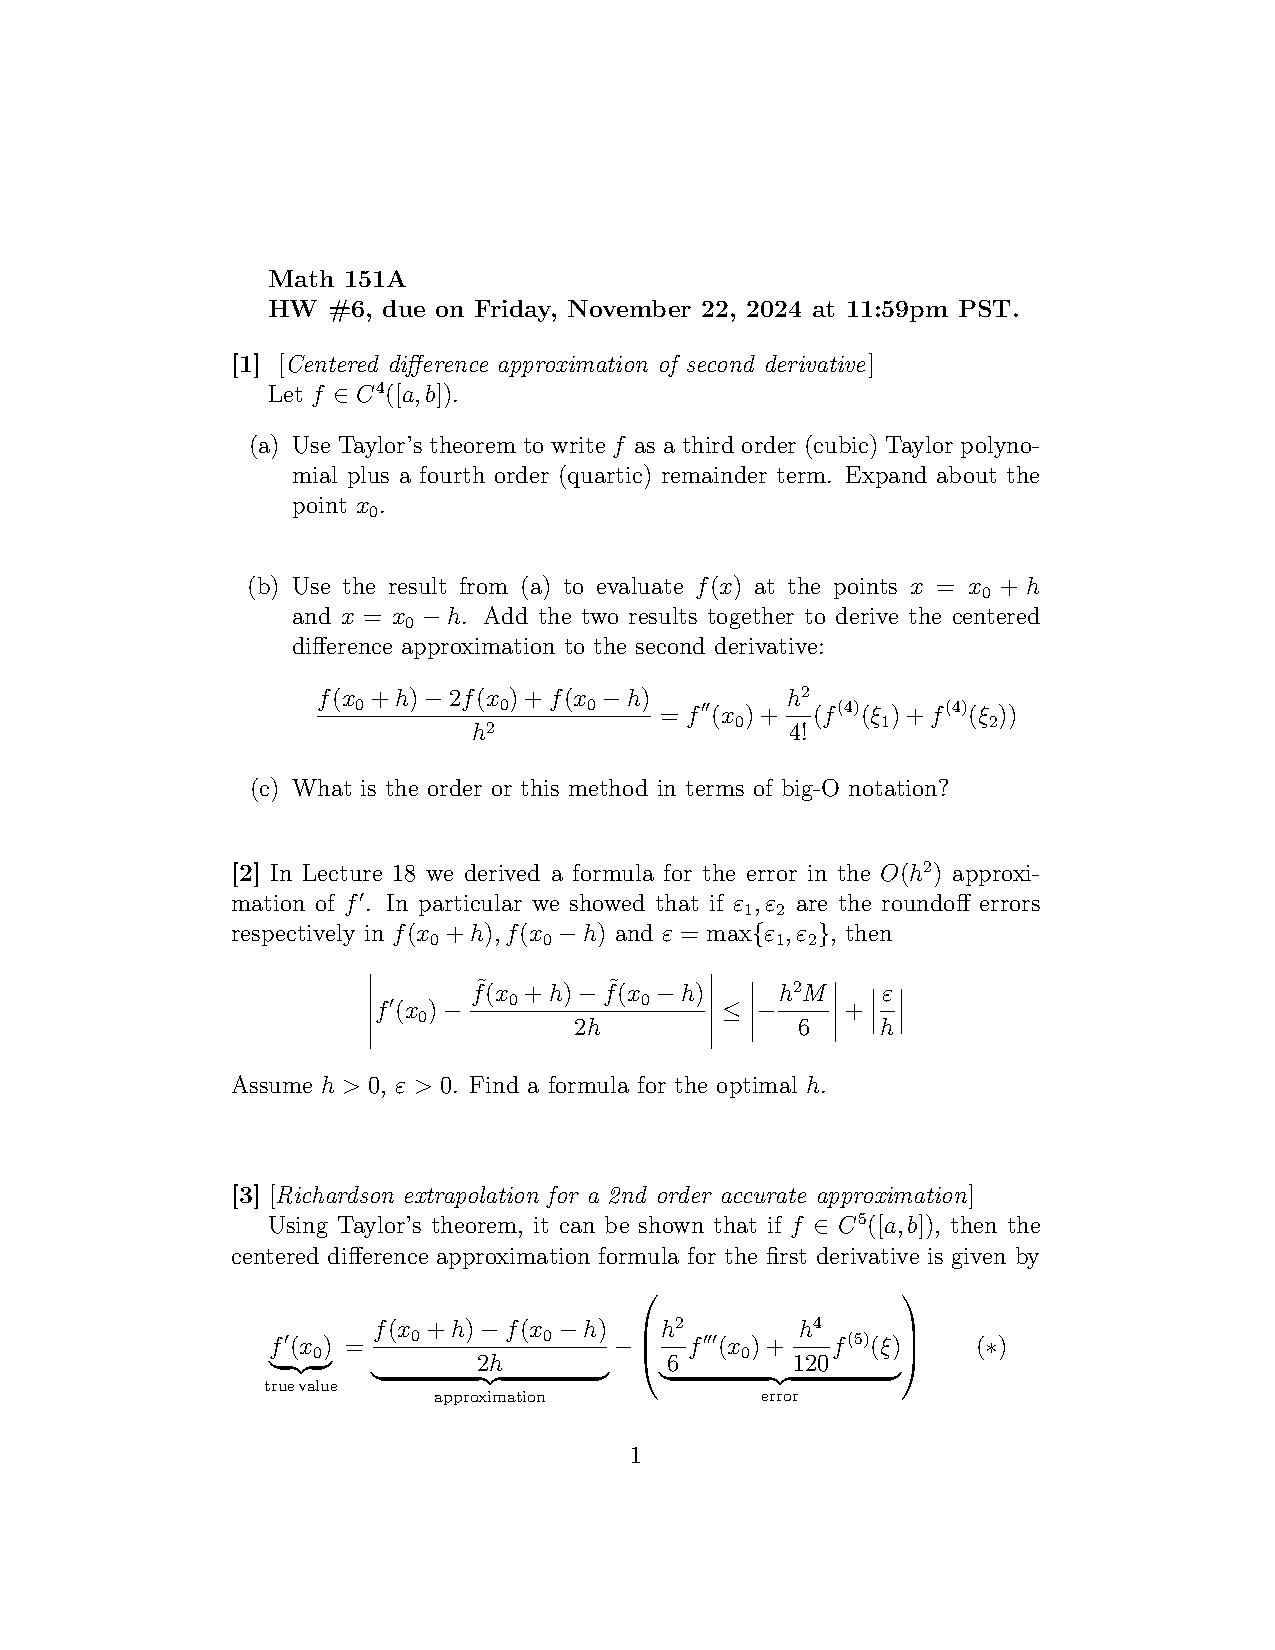
\includepdf[pages=-]{assignment.pdf}

\end{document}
